%% ****** Start of file aiptemplate.tex ****** %
%%
%%   This file is part of the files in the distribution of AIP substyles for REVTeX4.
%%   Version 4.1 of 9 October 2009.
%%
%
% This is a template for producing documents for use with 
% the REVTEX 4.1 document class and the AIP substyles.
% 
% Copy this file to another name and then work on that file.
% That way, you always have this original template file to use.

\documentclass[aip,rsi]{revtex4-1}
\usepackage{graphicx}
%\documentclass[aip,reprint]{revtex4-1}

%\draft % marks overfull lines with a black rule on the right

\begin{document}

% Use the \preprint command to place your local institutional report number 
% on the title page in preprint mode.
% Multiple \preprint commands are allowed.
%\preprint{}

\title{High Mass Resolution Time of Flight Mass Spectrometer for Measuring Products in Heterogeneous Catalysis in Highly Sensitive Microreactors} %Title of paper

% repeat the \author .. \affiliation  etc. as needed
% \email, \thanks, \homepage, \altaffiliation all apply to the current author.
% Explanatory text should go in the []'s, 
% actual e-mail address or url should go in the {}'s for \email and \homepage.
% Please use the appropriate macro for the type of information

% \affiliation command applies to all authors since the last \affiliation command. 
% The \affiliation command should follow the other information.

\author{T. Andersen}
\author{R. Jensen}
\author{M.K. Christensen}
\affiliation{Department of Physics, Danish National Research Foundation's Center for Individual Nanoparticle Functionality (CINF), Technical University of Denmark, Building 312, DK-2800 Kgs. Lyngby, Denmark}
\author{T. Pedersen}
\author{O. Hansen}
\affiliation{Department of Micro- and Nanotechnology, Technical University of Denmark, DTU Nanotech Building 345 East, DK-2800 Kgs. Lyngby, Denmark}
\author{I. Chorkendorff}
\email[]{ibchork@fysik.dtu.dk}
\affiliation{Department of Physics, Danish National Research Foundation's Center for Individual Nanoparticle Functionality (CINF), Technical University of Denmark, Building 312, DK-2800 Kgs. Lyngby, Denmark}
%\homepage[]{Your web page}
%\thanks{}
%\altaffiliation{}
%\affiliation{}

% Collaboration name, if desired (requires use of superscriptaddress option in \documentclass). 
% \noaffiliation is required (may also be used with the \author command).
%\collaboration{}
%\noaffiliation

\date{\today}

\begin{abstract}
We demonstrate a combined microreactor and time of flight system for testing and characterization of heterogeneous catalysts with high resolution mass spectrometry and high sensitivity. Catalyst testing is performed in silicon-based microreactors which have high sensitivity and fast thermal response. Gas analysis is performed with a time of flight mass spectrometer with a modified nude Bayard-Alpert ionization gauge as gas ionization source. The mass resolution of the time of flight mass spectrometer using the ion gauge as ionization source is estimated to m/$\Delta$m$>$2500. The system design is superior to conventional batch and flow reactors with accompanying product detection by quadrupole mass spectrometry or gas chromatography not only due to the high sensitivity, fast temperature response, high mass resolution and fast acquisition time of mass spectra but also allows wide mass range (0--5000\,amu in the current configuration). As a demonstration of the system we present data from ammonia oxidation on 5\,nm Pt nanoparticles showing resolved spectra of OH$^{+}$ and NH$_{3}^{+}$.
\end{abstract}

\pacs{}% insert suggested PACS numbers in braces on next line

\maketitle %\maketitle must follow title, authors, abstract and \pacs

% Body of paper goes here. Use proper sectioning commands. 
% References should be done using the \cite, \ref, and \label commands
\section{Introduction}
In heterogeneous catalysis optimization and development of equipment is important both to minimize the cost of equipment but also to be able to study complicated systems. As a platform for testing heterogeneous catalysts microfabricated reactors or microreactors have been found suitable due to both high surface-to-volume ratio, fast temperature response and minimization of thermal and concentration gradients\cite{Jensen2001,Jaehnisch2004}. Such a platform has been developed to test and characterize model catalysts in our department\cite{Henriksen2009}. However, a suitable reactor platform is only part of the task; reactant and product detection and characterization is essential to determine catalyst performance. Typically, quadrupole mass spectrometers (QMSs) are used in low pressure regimes to analyze gas composition while gas chromatographs (GCs) are used for high pressure measurements. The QMS, however, suffer from a low mass resolution (m/$\Delta$m$>\sim$m up to m$\sim$200) which makes analysis of complicated spectra difficult and cumbersome. The QMS is additionally subject to a low mass range (typically $\sim$100-200\,amu) limiting general use. Furthermore, QMSs are typically operated by logging a single (or a few) masses as a function of time to increase time resolution. This is at the expense of acquisition of full mass spectra during the experiment limiting operation by potentially losing interesting features in other masses not monitored. GCs have inherently low time resolution which make them unsuitable for fast time response measurements as in the case of microreactors and is in general difficult to use as mass spectrometers due to the difficult interpretation of complex mixtures. Furthermore, GCs samples only a very small part of converted gas making them unsuitable for small amounts of reactant and product gases due to the low sensitivity. As an alternative to GCs or QMSs time of flight mass spectrometers (TOF-MS) offer both high mass resolution ($\Delta$m/m$>$1000), fast acquisition of full mass spectra ($>$1\,Hz), high sensitivity making them suitable for very small amounts of catalyst, i.e. model systems, and mass range only limited by the detector. For standard available microchannel plate (MCP) as detector a mass range of 0--5000\,amu can be obtained. 

Typically TOF-MS in heterogeneous catalysis is used as a surface analytic tool, i.e. TOF-SIMS\cite{Benninghoven1994,DeSmet1998,Grams2004,Johnson2010}. Measurements of reactants and products on heterogeneous catalysts by TOF-MS have previously been performed\cite{Levy1963,Okumura2007} but, until now, to our knowledge, the testing of catalysts in a microreactor with subsequent gas analysis by a TOF-MS has not been demonstrated. Here we describe a microreactor and TOF-MS system which combines the high sensitivity of microreactors and the high mass resolution TOF-MSs for testing and characterizing of heterogeneous catalysts.

\section{System design}
The microreactor as a reactor platform and TOF-MS as mass spectrometer enables high sensitivity reactivity measurements of the catalyst under investigation combined with high resolution mass spectrometry. 

The catalyst under investigation is deposited in the microreactor reactor volume by e.g. evaporation\cite{Henriksen2009}, drop casting\cite{Vesborg2010} or gas aggregation formed size-selected nanoparticles. The gas composition in the microreactor reactor volume is ionized by the ion gauge and is subsequently detected by the TOF-MS which is connected to a capillary outlet on the microreactor. A schematic of the entire setup is shown in Figure \ref{fig:TOF_microreactor}.
\begin{figure}
 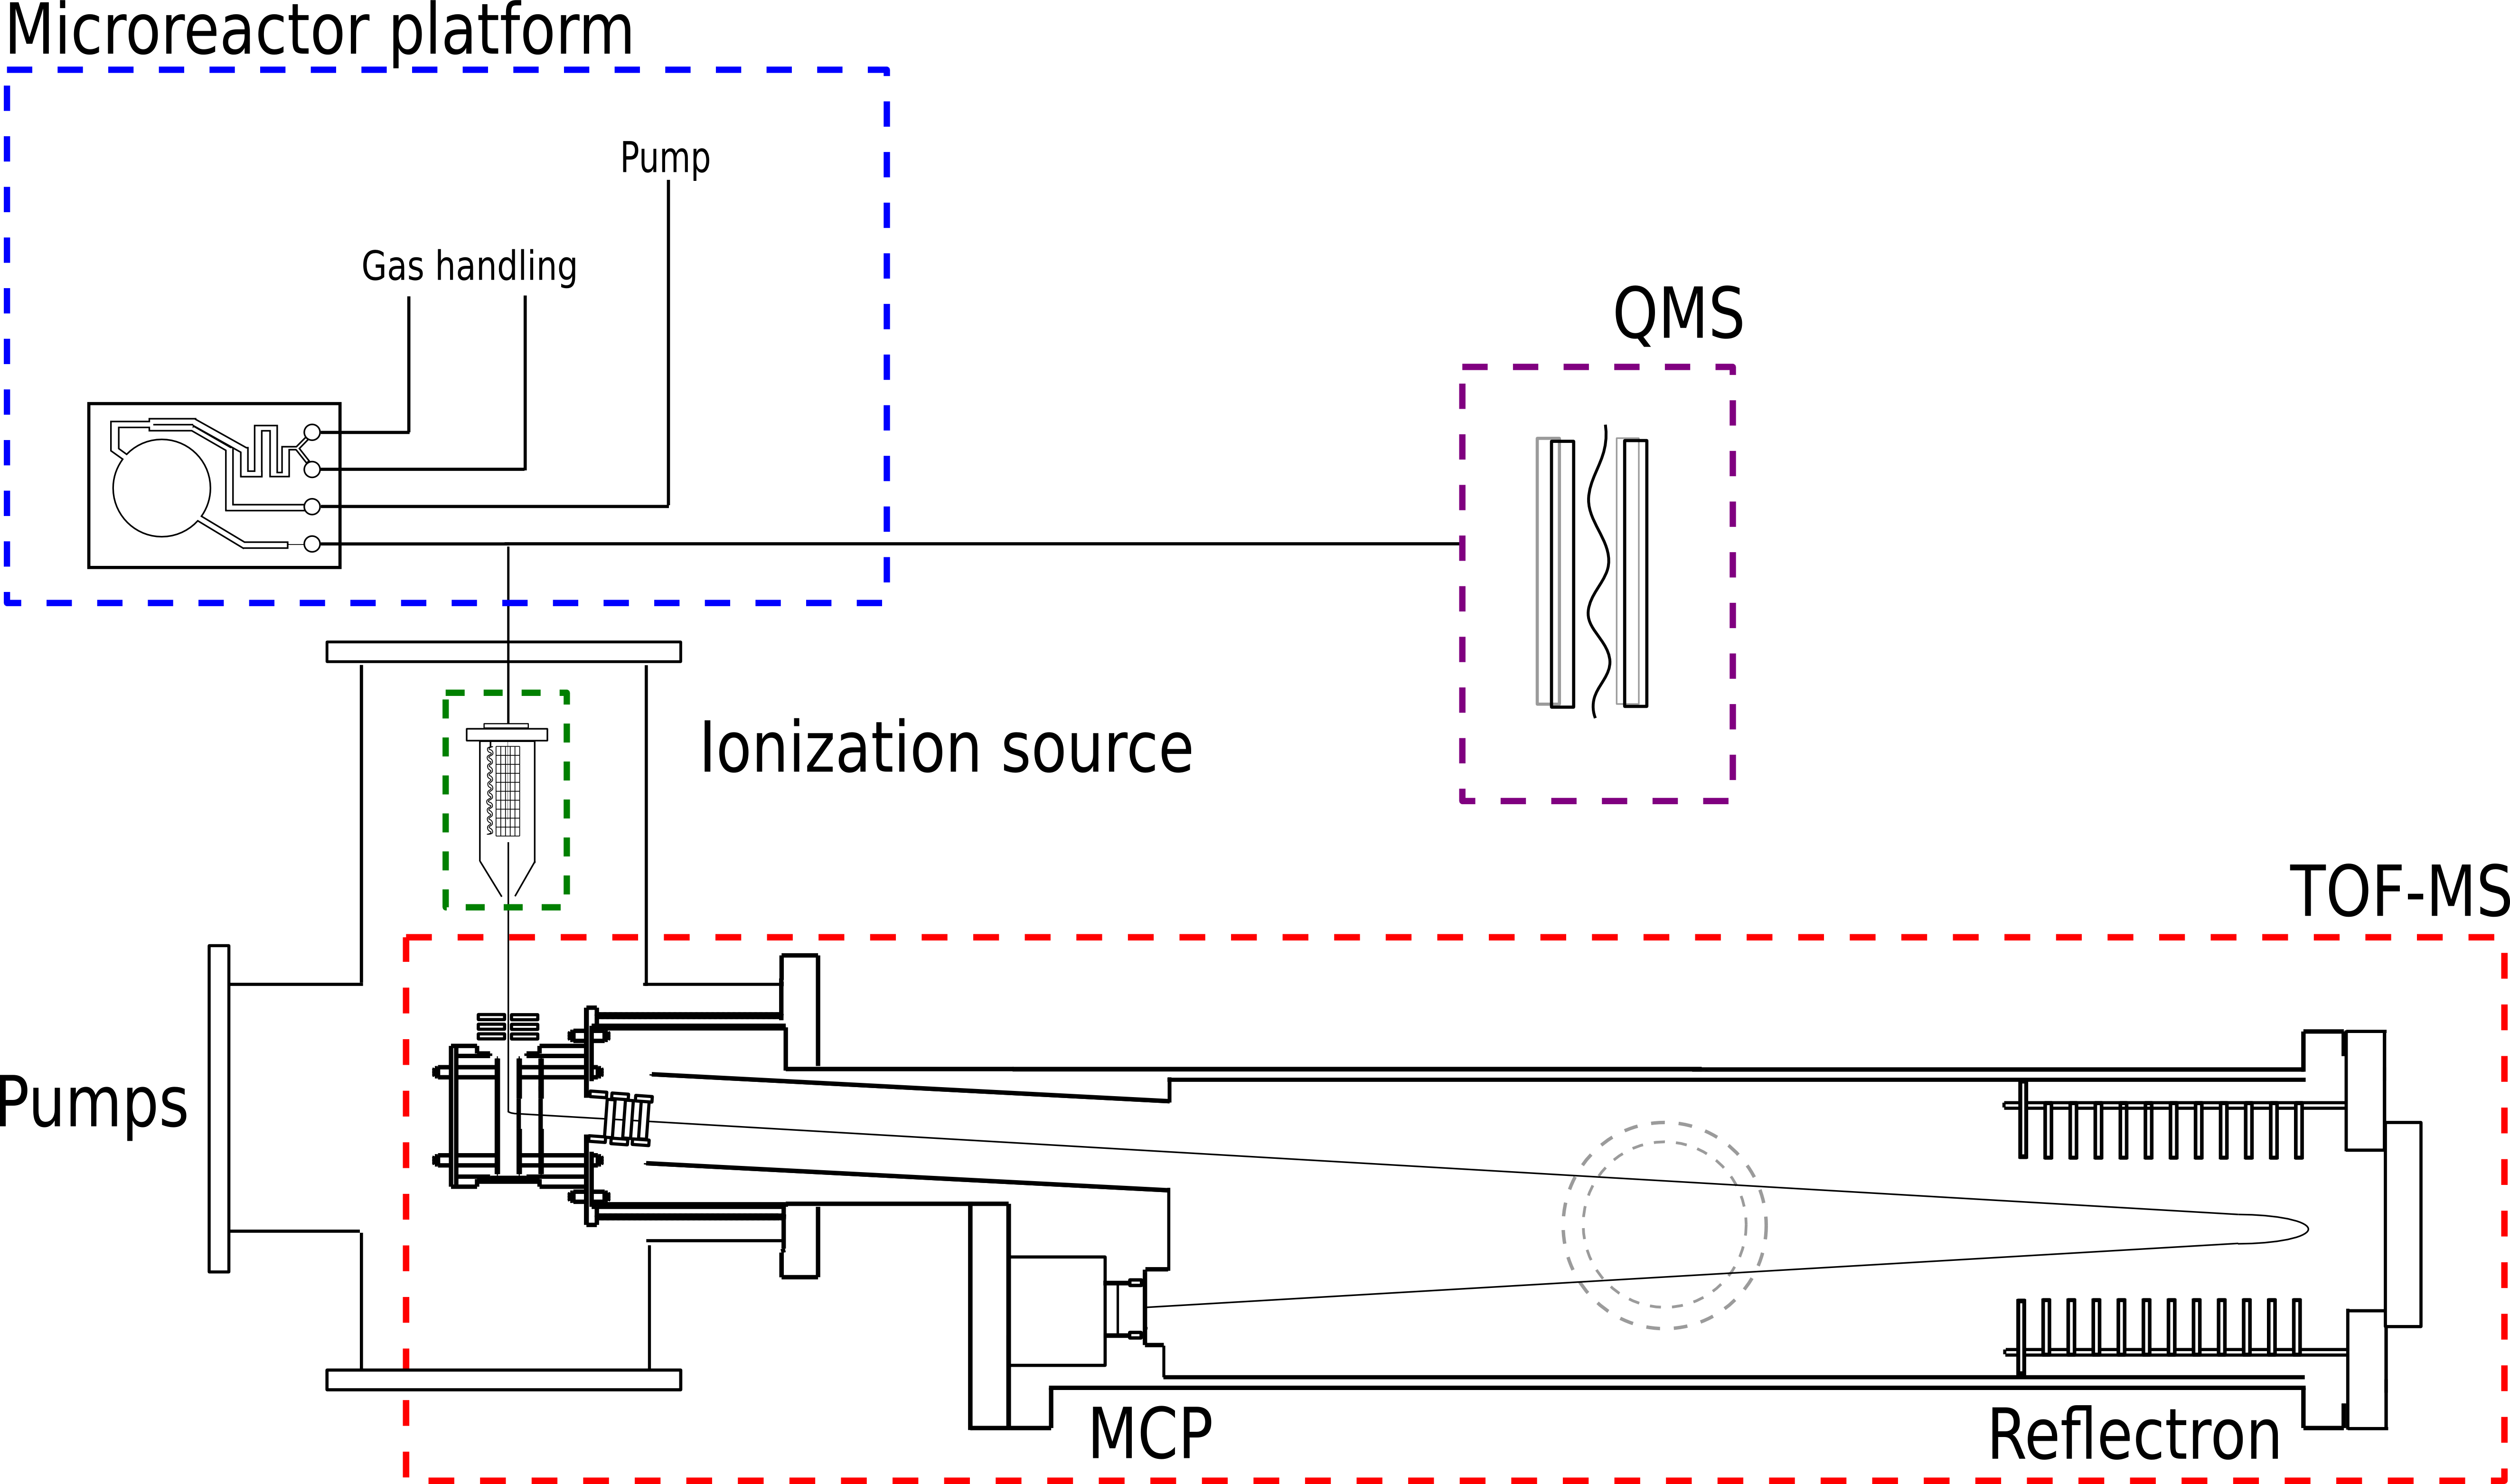
\includegraphics[width=14cm]{TOF_microreactor.png}%
 \caption{Schematic of the total system (not to scale). The capillary outlet from the microreactor can be directed to either a QMS or the TOF-MS. For measurements by the TOF-MS the gas is fed into a modified ion gauge which ionizes the gas. The ionized gas hereafter enters the TOF through a series of Einzel lenses from where they are pushed into the flight tube by a repelling voltage, V$_p$. After the focusing by the reflectron the ions are detected by a MCP.\label{fig:TOF_microreactor}}%
\end{figure}
The setup consists of three main components. The microreactor, where the catalyst under investigation is deposited, an ionization source which ionizes the gas from the microreactor and the TOF-MS used for gas analysis. A QMS is furthermore connected to the capillary of the microreactor which enables direct comparison between the QMS and TOF-MS.

\subsection{The microreactor platform}
Catalyst characterization and performance evaluation is performed in a microreactor platform \cite{Henriksen2009}. The microreactors are silicon-based and measures 20x15\,mm. The reactor consists of two gas inlets, a gas outlet, a reactor volume and a capillary used to restrict the gas flow from the reactor volume. The reactor volume is 3\,$\mu$m deep and 1 cm in diameter corresponding to a 236\,nL. The diffusion length of the reactants and products gases in the microreactor reactor volume is almost an order of magnitude longer than the radius of the reactor volume ensuring full contact of the gas with the catalyst. This has been proven to hold by reproducible CO oxidation on Pt spots located at different points in the the reactor volume. The two gas inlets are combined on the chip where the inlet gases mix by diffusion. The capillary is designed such that approximately $3\times10^{14}$\,molecules$\cdot$s$^{-1}$ is probed from the reactor volume when operated at 1\,bar. Any surplus of gas from the two inlets that does not enter the reactor volume is directed through an outlet to a turbo pump. The design ensures that all molecules or atoms entering the reactor volume, hence exposed to the catalyst under investigation, is detected by mass spectrometry ensuring high sensitivity. 

The microreactor is heated by joule heating of a 50\,nm platinum strip evaporated through a shadow mask on the backside of the chip. The heating element is contacted by two pogo pins which is connected to a power supply. Additionally, two extra contacts are placed on the chip facilitating a 4 wire measurement of the resistance of the heating element. The heating strip can in this way be used as a resistance temperature detector (RTD) to determine the temperature of the chip. At the current configuration temperatures from room temperature to approximately 450\,$^{\circ}$C can be reached.


\subsection{Gas handling for the microreactor}
The two gas inlets on the microreactor chip is connected to a gas handling system. A total of 6 gases with accompanying flow controllers are used to control the inlet gas flow to the microreactor. Currently, the system is configured in a 4+2 setup where 4 gases are connected to the first inlet and two gases connected to the secondary inlet. At the time of writing He, CO, O, CH$_4$, NH$_3$ and H$_2$. All gases used on the setup are N6 quality gases, i.e. 99.9999\,\% purity. All valves and flow controllers are interfaced to computer enabling remote control of the system and the ability to run experiments over several days without human intervention.

\subsection{Time of flight mass spectrometer}
The time of flight chamber is pumped by a turbo pump and two ion pumps. A 120\,l/s ion pump is used to pump the flight tube while a 400\,l/s ion pump and a 450\,l/s turbo pump is used to pump down the source region which is mounted on a 8" 4-way cross. Opposite the source region of the TOF-MS the pumps are mounted while the two remaining flanges are occupied by the ionization gauge and a blanked flange (see Figure~\ref{fig:TOF_microreactor}). While idling the pressure in the source region is $\sim1\cdot10^{-9}$\,mbar and $\sim2\cdot10^{-9}$\,mbar in the flight tube.

The time of flight equipment used for detection of gas molecules flowed through the capillary of the microreactor is designed as an orthogonal mass spectrometer and is assembled from modules purchased from Jordan TOF Products, Inc\cite{JordanHomepage}. 

Ionized ions enter the source of the TOF-MS through a series of entry Einzel lenses used for focusing the beam hence minimizing divergence. In the source the beam is pushed into the flight tube by an the initial repelling push voltage, $V_p$. The ions are further accelerated from ground potential to the liner potential, $V_L$. Using this setup the drift velocity of an ion starting exactly from the center of the acceleration region is $V_L + V_p/2$. At the end of the flight tube a reflectron is installed which is controlled by voltages $V_{R1}$ and $V_{R2}$. The reflectron has two primary purposes: i) The effective drift length is increased hence increasing resolution of the TOF-MS. ii) The reflectron works as a focusing lens compensating for any initial velocity dispersion of the ions, i.e. ions with an initial higher velocity will have an increased flight length compared to slower ions. The MCP used for ion detection is placed in the focal point of the reflectron giving maximum compensation for initial velocity dispersion. According to the manufacturer a resolution m/$\Delta$m$>\sim$4000 of the TOF has been shown.

The prize of the TOF including ionization, 8" 4-way cross, control electronics, data acquisition hardware and MCP detector is estimated to USD80.000 which is comparable to a high quality QMS which is prized at approximately USD85.000.

In Figure \ref{fig:untreated_data} an example spectrum of a methanol and atmospheric air mixture is shown. Here the high resolution of the TOF-MS is demonstrated by resolving methanol (CH$_3$OH) and molecular oxygen (O$_2$) which have a mass difference of 43\,milli-amu.
\begin{figure}
 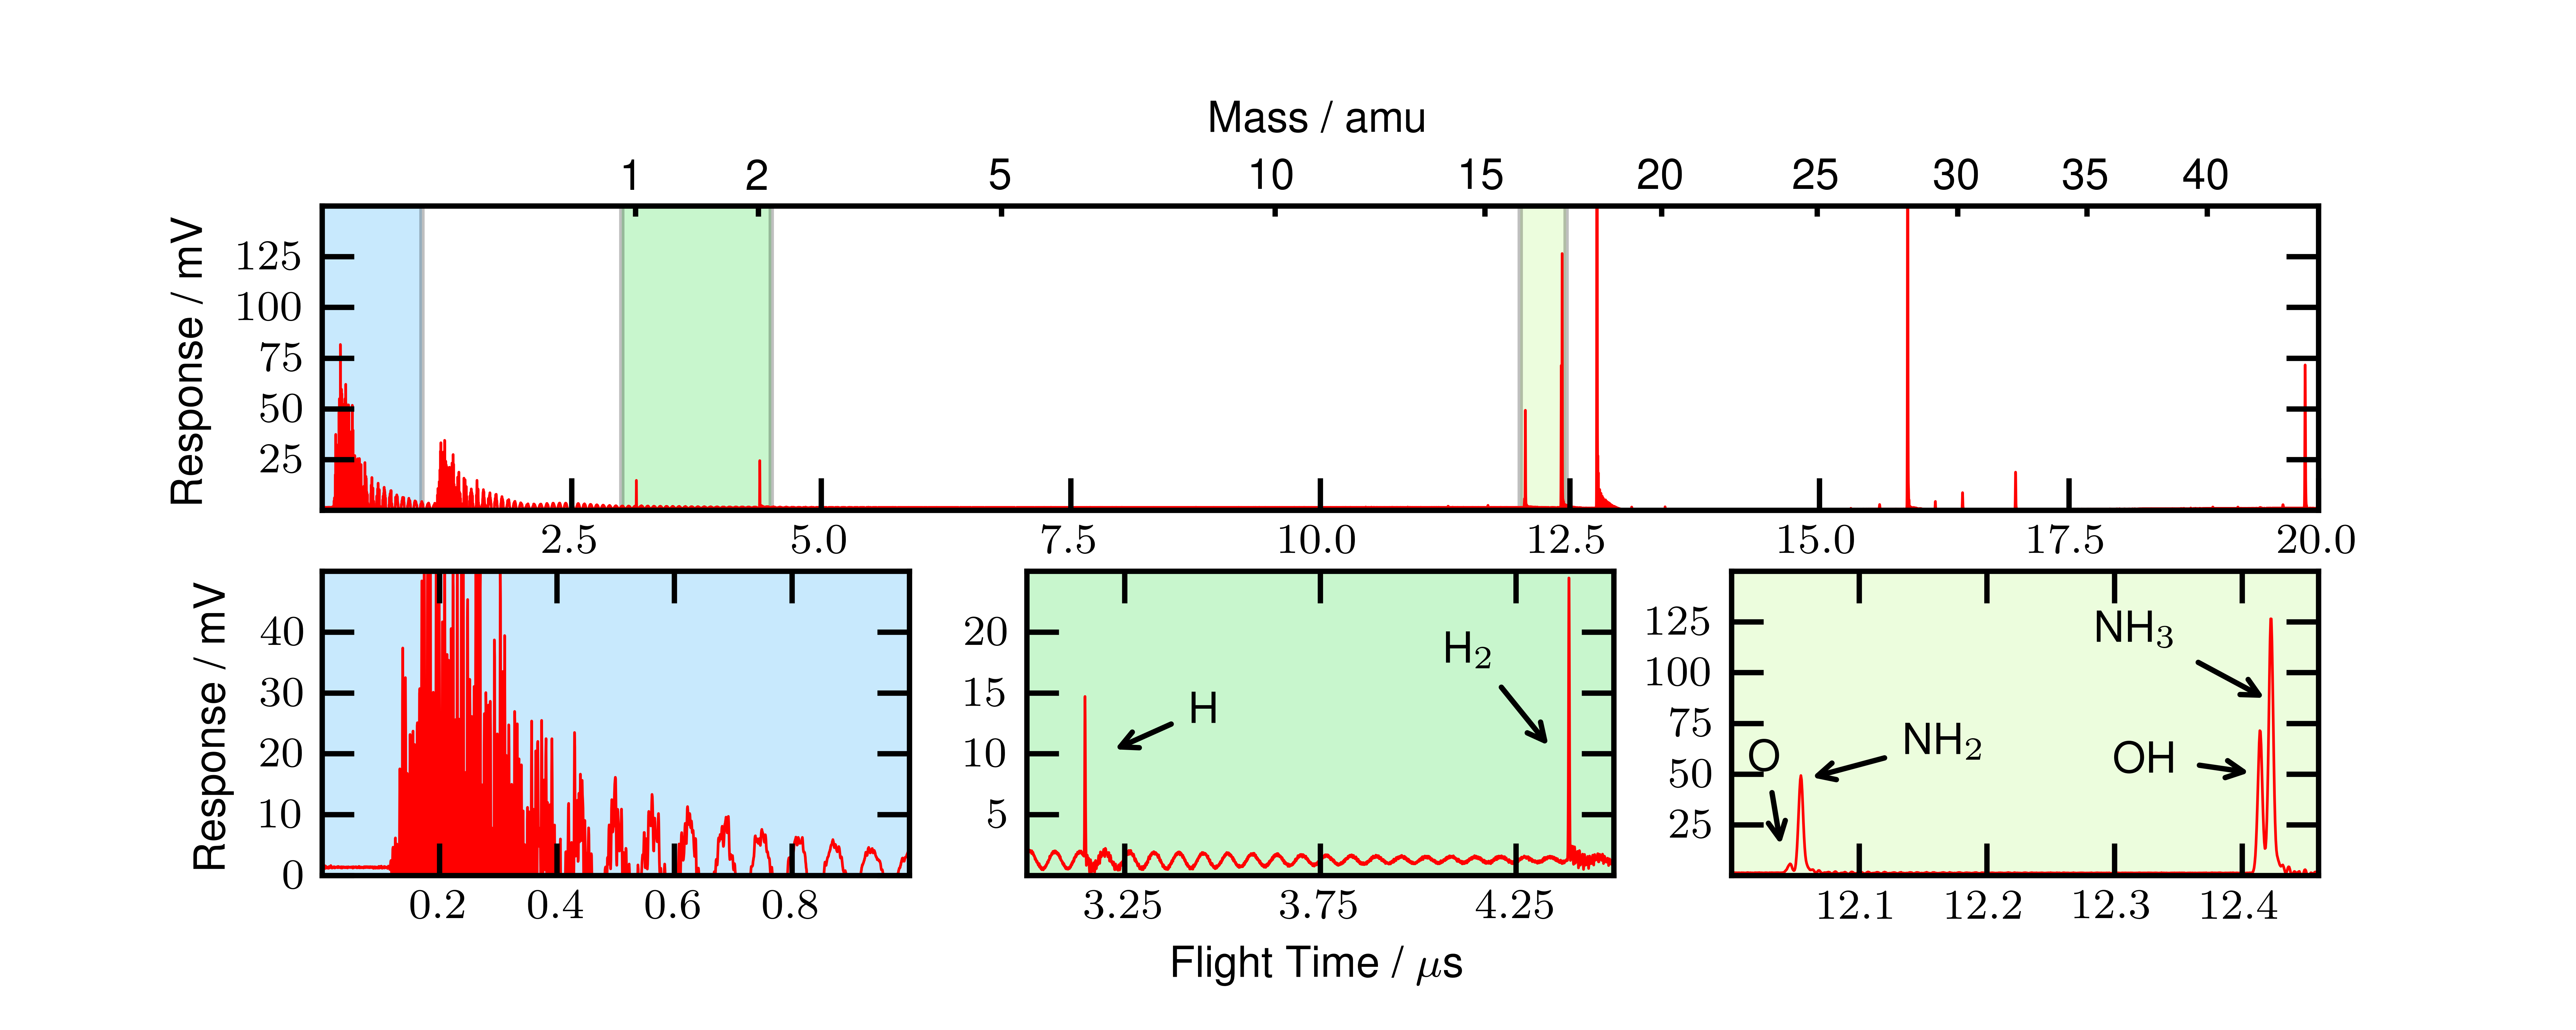
\includegraphics[width=16cm]{untreated_data.png}%
 \caption{Raw data acquired from the TOF-MS in a gas mixture of methanol and atmospheric air. Subfigures show three different regions of the spectrum. From the first subfigure a delay of approximately 150\,ns can be seen due to delays in cables and the rise time of the repeller pulser. In the center subfigure the extremely good seperation between masses is shown. It is evident that 1\,amu corresponds to approximately 350\,ns difference in flight time in our system in the mass regime around 20\,amu. In the last subfigure a zoom of the methanol and molecular oxygen (43\,milliamu mass difference) region is shown.\label{fig:untreated_data}}%
\end{figure}

\subsubsection{Ionization of gas}
As ionization source of the gas flow from the microreactor capillary a modified nude UHV Bayard-Alpert ion gauge is used. 3\,A is run through the filament resulting in 10\,mA emission current. The grid is biased approximately 40\,V negative compared to the filament to accelerate electrons emitted from the filament towards the grid. Contrary to standard operation of an ion gauge the collector in the center of the grid is short-circuited to the grid ensuring homogeneous field distribution within the grid. To allow ionized ions to escape from the gauge the lid of the grid has been removed. Using this configuration approximately half of the ionized ions are expected to leave the ionization gauge\cite{Nottingham1955}. The entire construction is placed in a nozzle which is differentially pumped by a turbo pump. Large amounts of gas can hence be dosed locally around the ion gauge while still maintaining a low pressure in the source region of the TOF-MS. The nozzle is essential in the setup to avoid high pressure in the acceleration region and drift tube resulting in an increase in dead counts on the MCP thus decreasing the signal-to-noise ratio of the recorded signal.

\subsubsection{Data treatment}
Raw data plotted with accompanying gaussian fits are shown in Figure \ref{fig:gaussian_fit}. Here the closely lying peaks from OH$^{+}$ from cracking of both residue water and water as reaction product and uncombusted NH$_3^{+}$ is shown. The ability to separate these contributions substantially simplifies quantification of ammonia and allows for easier characterization of catalyst performance. 
\begin{figure}
 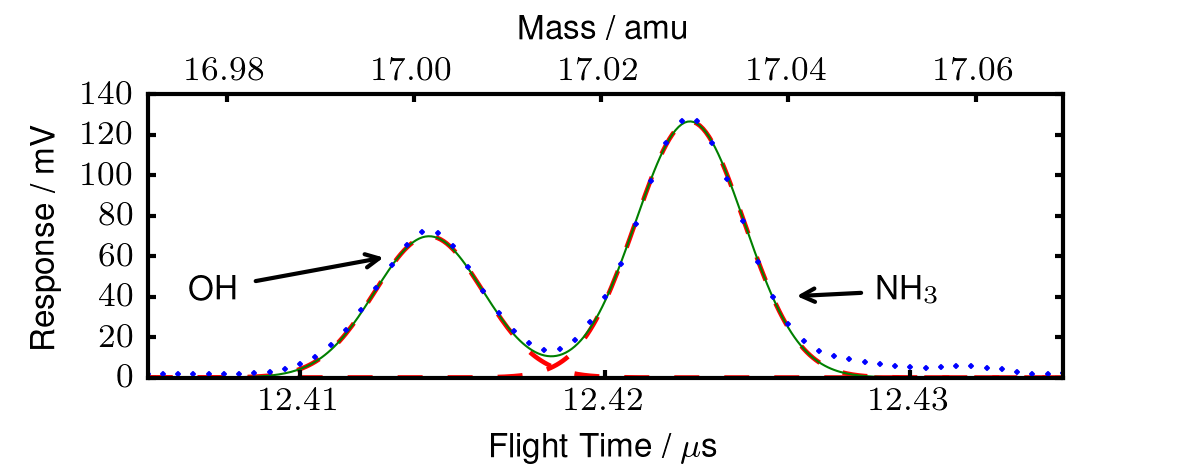
\includegraphics[width=14cm]{ammonia_OH_gauss_fit.png}%
 \caption{Example of two gaussian fits (dashed red lines) and the sum of the two fits (green solid line) to a double peak consisting of NH$_{3}^{+}$ and OH$^{+}$ both at approximately 17\,amu demonstrating the resolution of the TOF-MS. The entire graph section represents a mass difference of 100\,milli-amu.\label{fig:gaussian_fit}}%
\end{figure}
In Figure \ref{fig:dynamic_range} raw data from water, hydrogen and oxygen from three different regions is shown illustrating the dynamic range of the TOF-MS. At constant MCP voltage all the peaks are clearly visible although the ratio of the oxygen to water amplitude is $\sim$400. 
\begin{figure}
 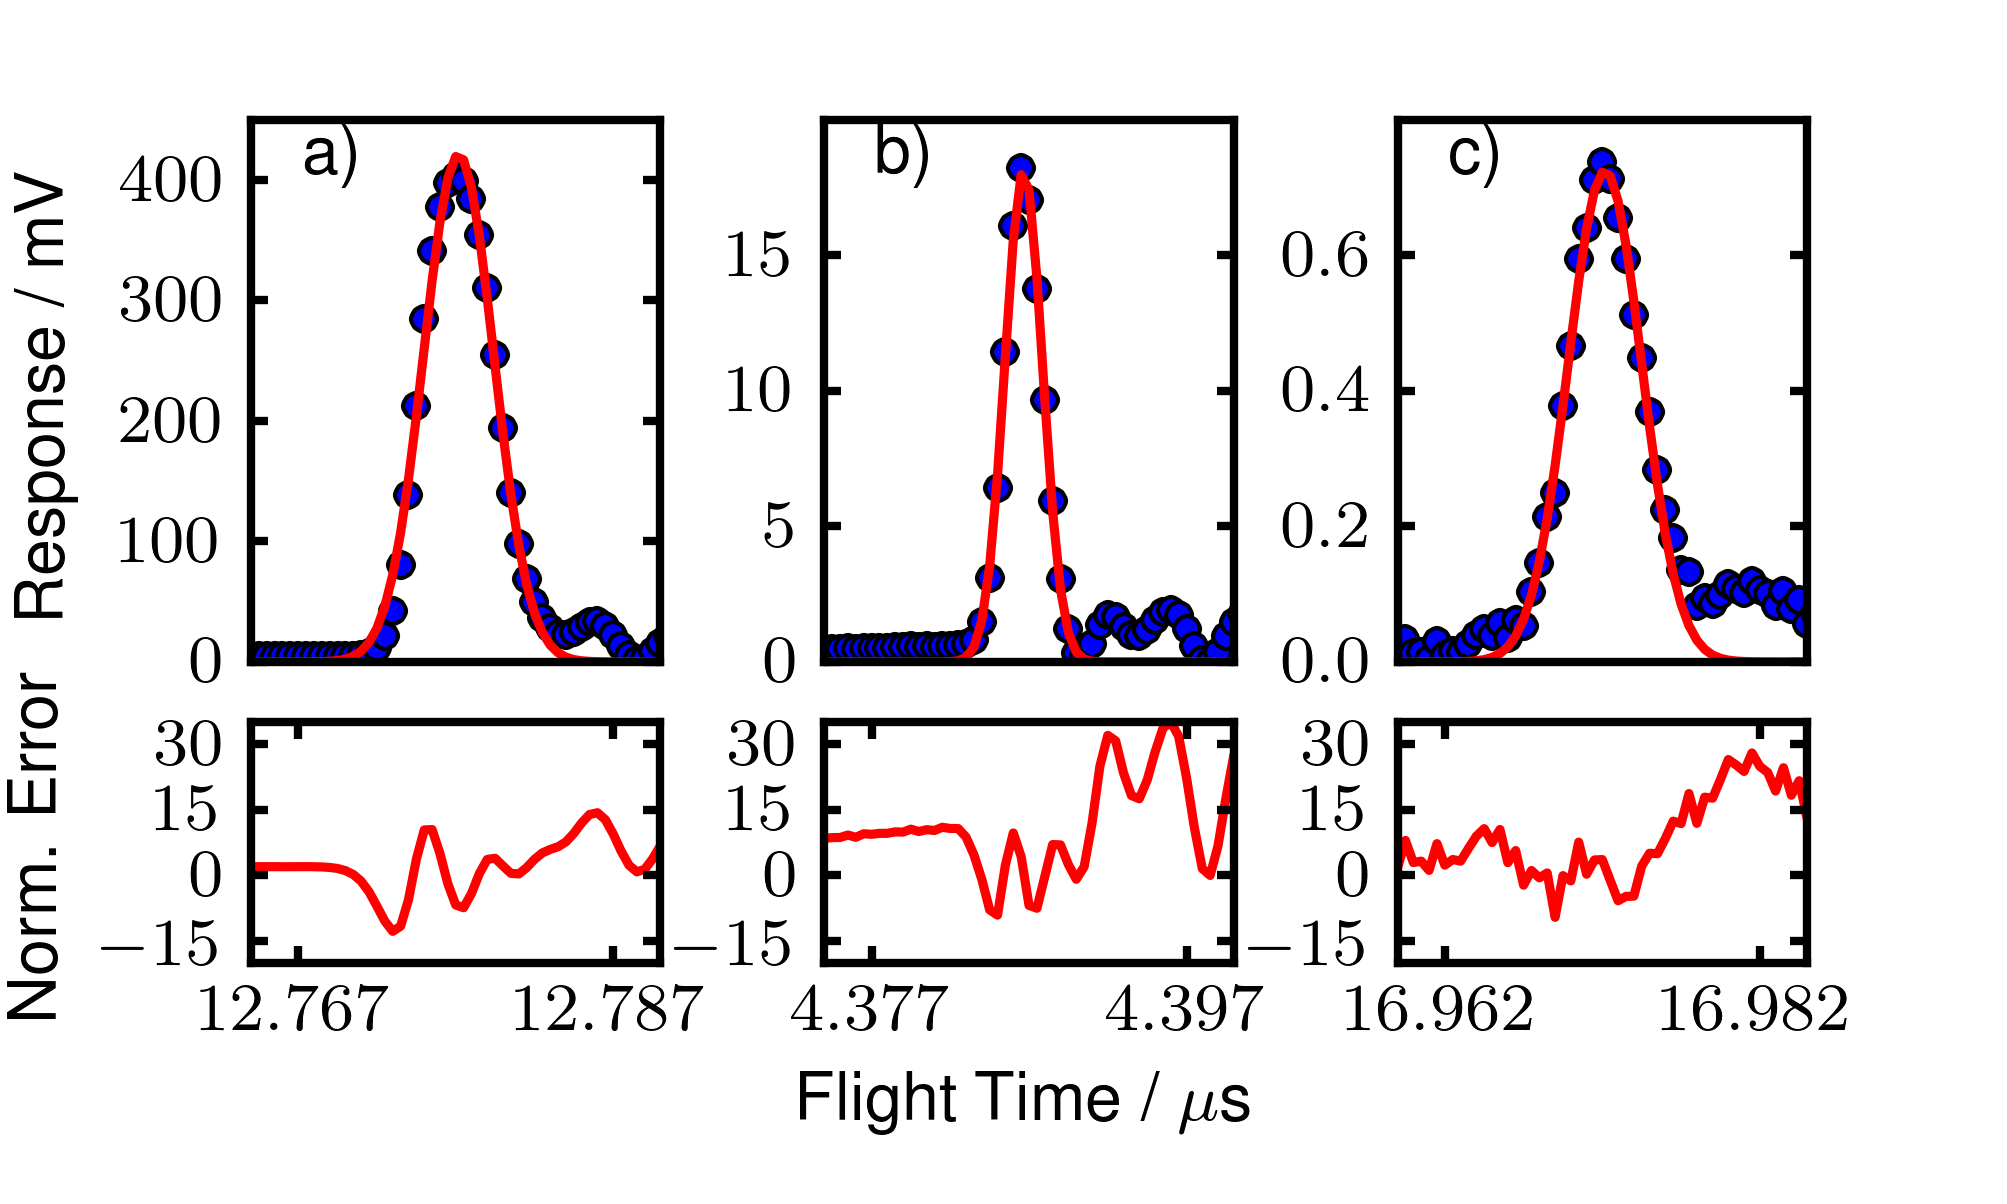
\includegraphics[width=14cm]{dynamic_range.png}%
 \caption{Gaussian fits to three different mass to charge ratios from the same mass spectrum (integrated area indicated in each panel). As seen from the response a high dynamic range of the TOF-MS all yielding good gaussian fits. The TOF-MS can hence be used to monitor both very small and very large signal masses with high time resolution.\label{fig:dynamic_range}}%
\end{figure}
In reality the dynamic range is limited mostly by the data acquisition hardware as well as the quality of the ion source. Even with the home-built ionization source and a 8-bit digitizer the dynamic range is from Figure~\ref{fig:dynamic_range} estimated to $\sim$1000 using an integration time of $\sim$5\,s. The dynamic range of the TOF-MS is hence comparable to the dynamic range offered by a QMS at constant preamplifier range while covering a much larger mass range.

Since the TOF-MS only measures flight time and not the actual mass of the measured molecules or atoms it is necessary to determine the relationship between flight time and actual mass. This can be done by calibration masses expressing known patterns in the mass spectrum. In this way masses can be reasonably determined with subsequent fitting of these values to get an expression for the flight time as a function of mass. This approach is in some cases adequate but does have the significant drawback that several peaks of well known masses must be present in the flight spectrum which is not always necessarily the case. To determine the relationship between mass and flight time we have made a numeric model of the mass spectrometer which calculates the flight time based only on the voltages for the pulser, $V_p$, liner, $V_L$, and reflectron, $V_{R1}$ and $V_{R2}$, and thus provides a relationship of flight time to mass. Typically, the model is used together with the experimental determination of a single mass since this will help fix the unknown delays originating from the measurement trigger, rise time of the high-voltage pulse at the repeller plate and cable delays. As seen in Figure~\ref{fig:model_error} the performance of the model is good despite its simplicity giving a total error in flight time estimation of $\sim$100\,ns at 70\,amu. The model is written in Python and can be acquired online\cite{ModelGithub}.
\begin{figure}
 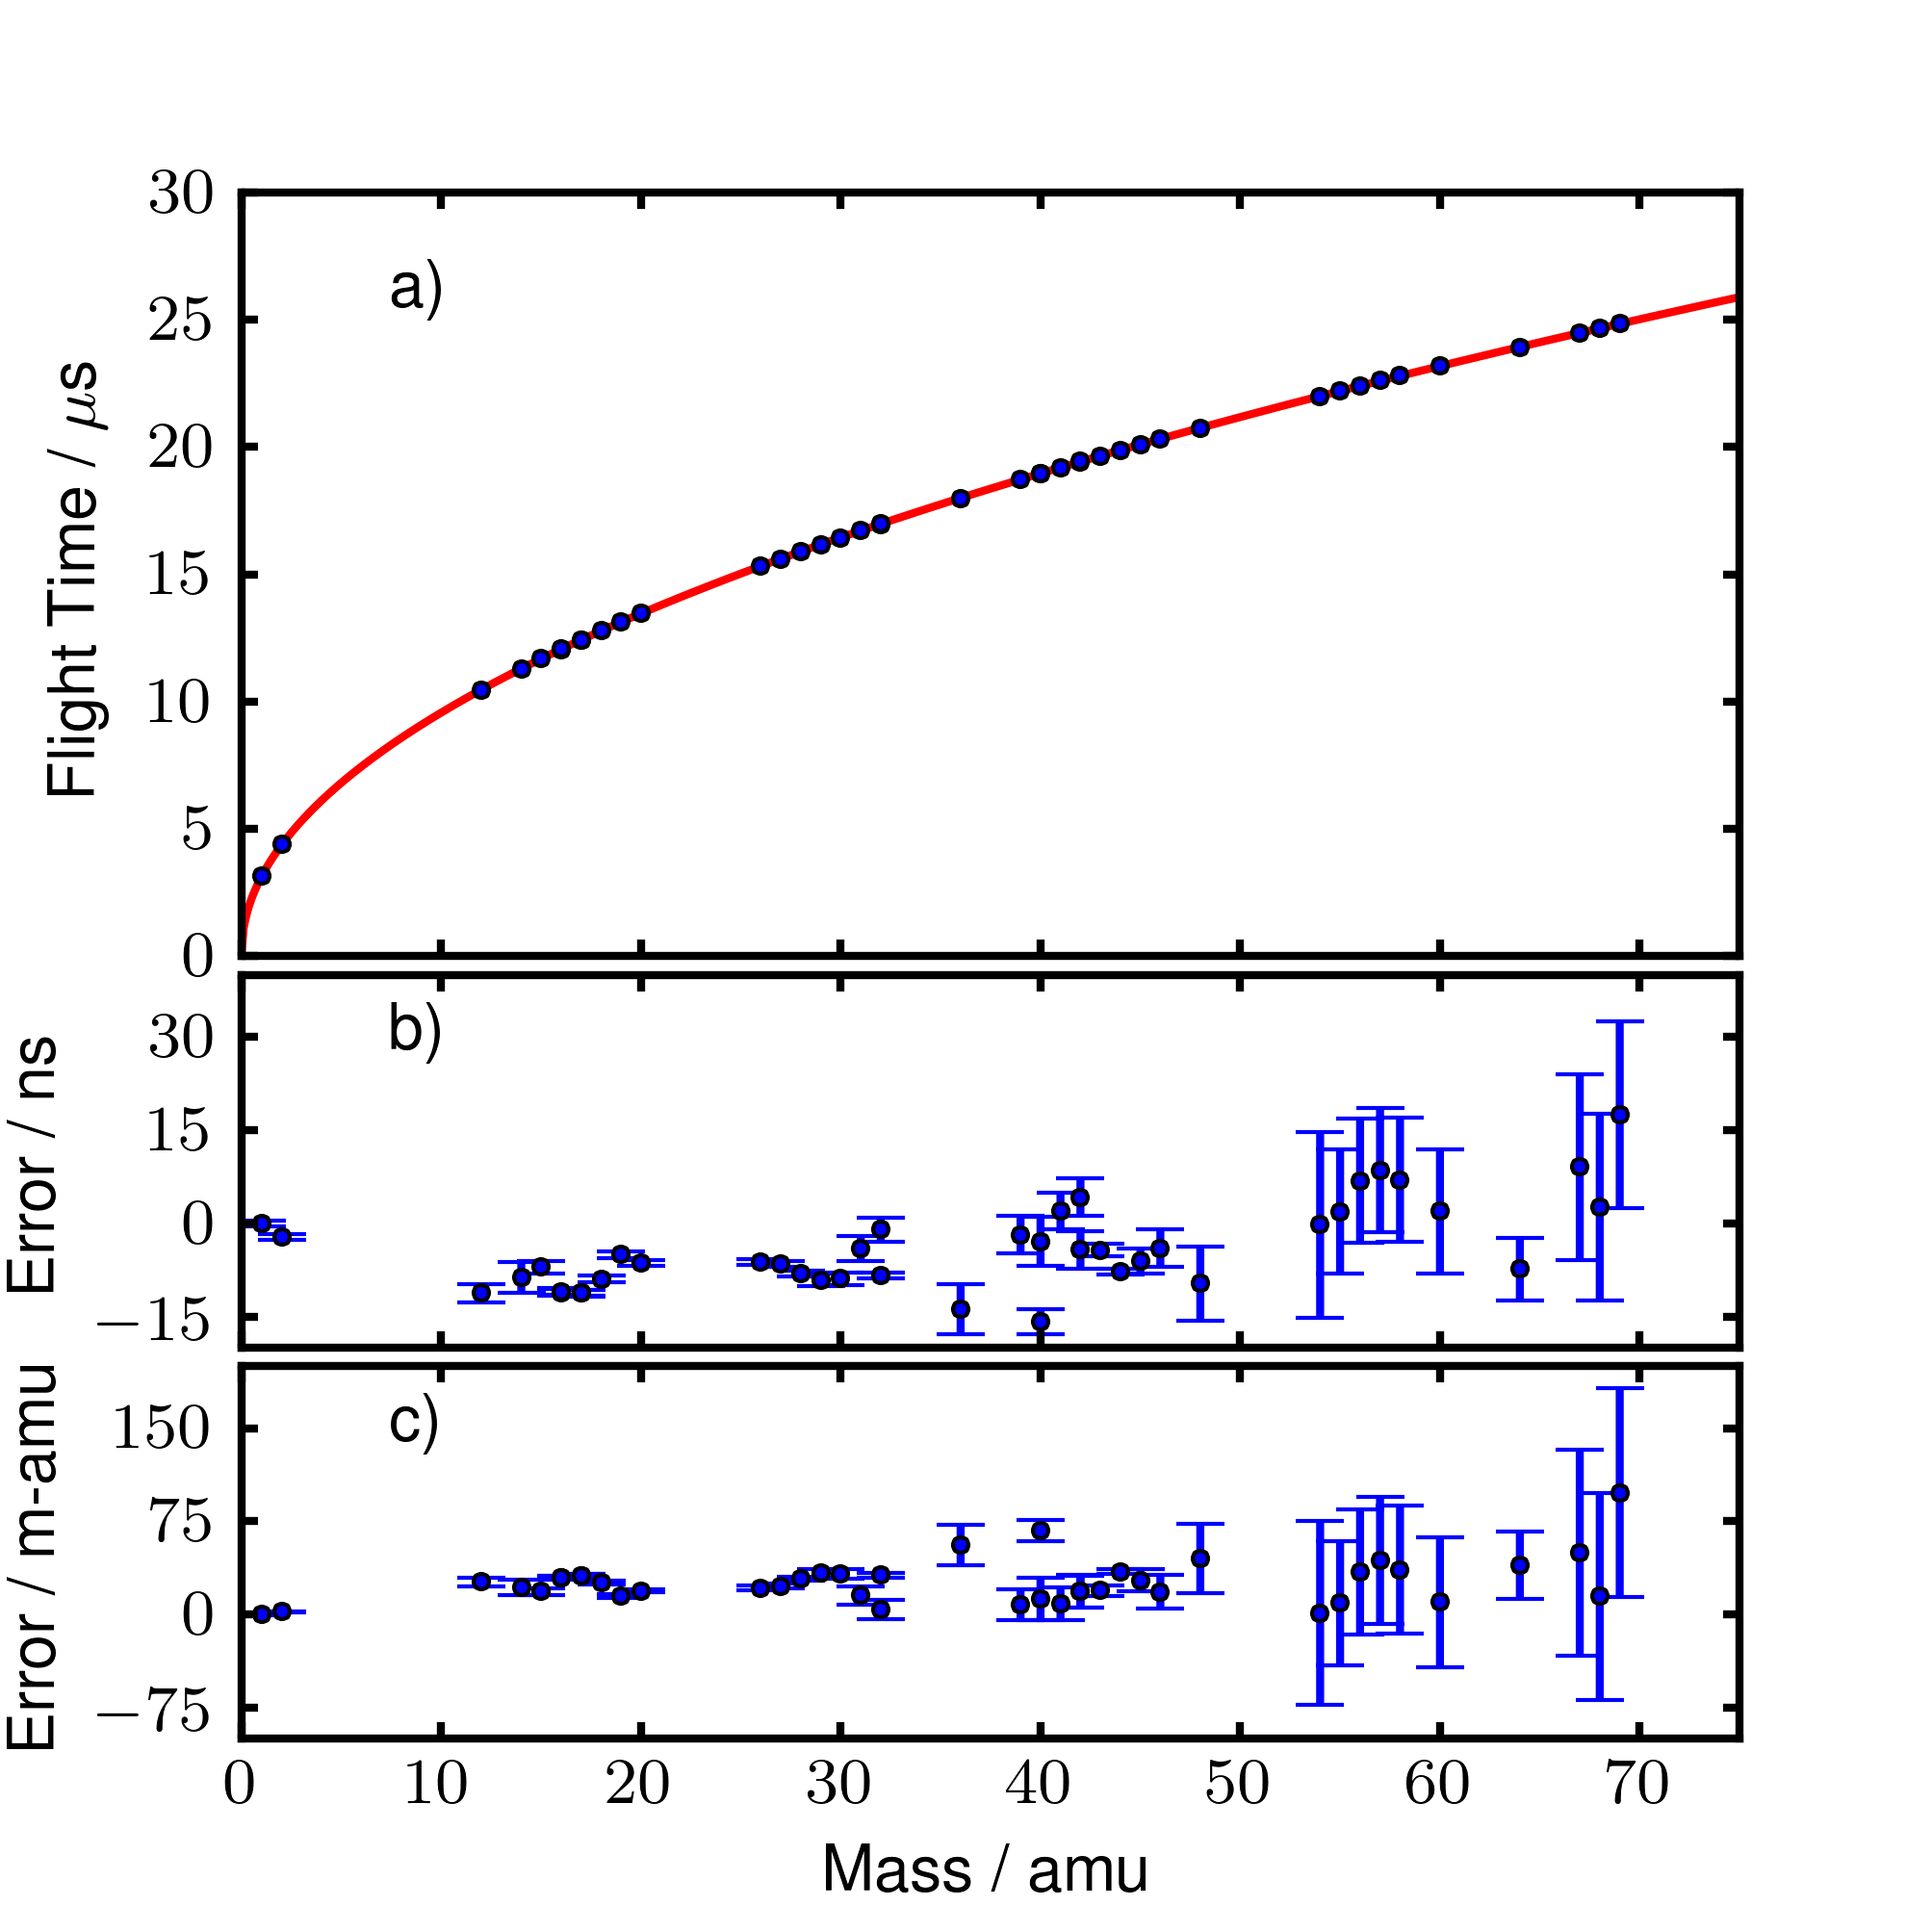
\includegraphics[width=14cm]{model_error.png}%
 \caption{Comparison of the simulated model (red line, top panel) to actual measured experimental values (blue dots). In the bottom panel the difference between acquired experimental data and data calculated from the model is plotted, errorbars represents only the uncertainty in the experimental data. As seen from the figure a deviation of $\sim$100\,ns at 70\,amu is present.\label{fig:model_error}}%
\end{figure}

\section{Oxidation of ammonia}
To demonstrate the system capability ammonia oxidation on a 40\,\% geometrical coverage 5\,nm Pt nanoparticles has been used as test reaction. The catalytic oxidation of ammonia can proceed along primarily three different routes.
\begin{equation}
4NH_3+3O_2\rightarrow 2N_2 + 6H_2O
\label{eq:Pt_clean_combustion}
\end{equation}
\begin{equation}
2NH_3+2O_2\rightarrow N_2O + 3H_2O
\end{equation}
\begin{equation}
4NH_3+5O_2\rightarrow 4NO + 6H_2O
\end{equation}
All of these systems are difficult to analyze both qualitatively and quantitatively due to the overlap of NH$_3$, which is a reactant, and OH$^+$ originating from cracking of H$_2$O, which is a product from the combustion and is a part of the residue gas. Specifically, hydroxyls (OH$^{+}$) from cracking of trace water in the system and the combustion reaction and the primary peak of ammonia (NH$_{3}^{+}$) are both detected at m/q$\simeq$17. Without adequate mass resolution it is not possible to separate the two contributions resulting in difficult analysis. Often a charge to mass ratio without cracking from either products or residue gas in the system is used to quantify the amount of ammonia and water. In the case of ammonia, m/q=15 or m/q=8.5 is typically chosen since water does not contribute to these masses. However, both of these masses contains only a very small fraction of the main peak since it involves either the loss of two hydrogen atoms or a double charged ammonia molecule which are processes with very low yields. The measurement of these masses have a very poor signal to noise ratio making measurements on ammonia very difficult with traditional mass spectrometry methods.

At experiment start the microreactor is equilibrated with NH$_3$ and O$_2$ in a 4:3 ratio corresponding to stoichiometry for this reaction. After equilibration the temperature is increased in steps of ?? from room temperature to 190\,$^{\circ}$C. The gas composition in the microreactor is continuously probed by the TOF-MS which is connected to the capillary of the microreactor.
\begin{figure}
 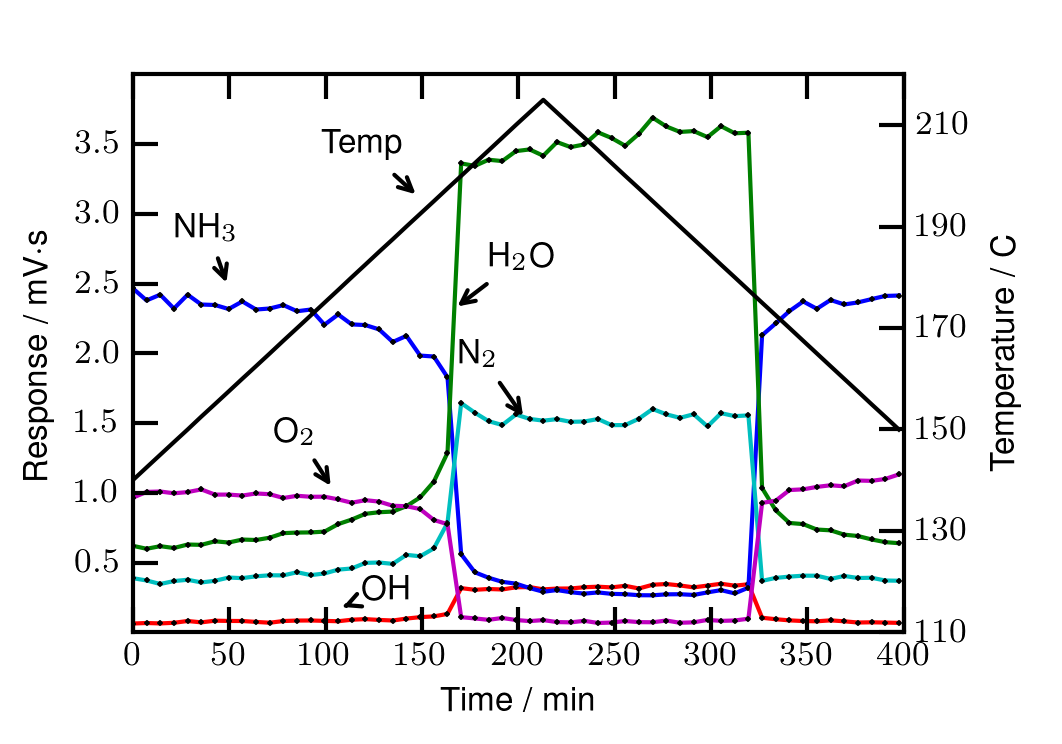
\includegraphics[width=14cm]{ammonia_reactivity.png}%
 \caption{Ammonia oxidation as a function of temperature on a 40\,\% geometrical coverage 5\,nm Pt nanoparticles. As the temperature is increased ammonia is oxidized to H$_2$O and N$_2$. Furthermore, the OH and NH$_3$ signal is anticorrelated demonstrating the ability to resolve these two close lying masses as shown in Figure \ref{fig:gaussian_fit}.\label{fig:ammonia_reactivity}}%
\end{figure}
In Figure~\ref{fig:ammonia_reactivity} the integrated N$_2$, NH$_3$, H$_2$O, O$_2$ and OH peaks acquired from the raw TOF-MS spectrum as a function of temperature are shown. At each individual temperature step a mass scan is performed from triggering of the acceleration pulse up to 25\,$\mu$s of flight time corresponding to 70 amu. As seen from Figure~\ref{fig:ammonia_reactivity} the combustion of NH$_3$ increases substantially at approximately 140\,$^{\circ}$C. The combustion of ammonia to molecular nitrogen and water at this temperature agrees well with literature\cite{Imbihl2007,Zeng2009}. 

In Figure \ref{fig:ammonia_reactivity} an anticorrelation between OH$^{+}$ and NH$_3^+$ is seen. The inverse relation between these two masses can only be measured because these peaks are resolved in the mass spectrum. As expected a strong correlation between H$_2$O$^{+}$ and OH$^+$ is seen as a direct result of water cracking to hydroxyls. The data shown in Figure~\ref{fig:ammonia_reactivity} hence demonstrates the usability of the combined microreactor and TOF-MS setup especially simplifying data analysis of complicated mass spectra while maintaining a high sensitivity from the microreactor platform.

%BØR VI LAVE ET ARRHENIUS PLOT??
%For ammonia oxidation both N$_2$O (m/q = 44), NO (m/q = 30) and NO$_2$ (m/q = 46) are of interest. 

\section{Summary}
We have demonstrated a combined microreactor and TOF-MS system which can be employed to test and characterize model heterogeneous catalysts. An automated gas handling system is used to flow gas over a catalyst in a microreactor volume from where gases can be probed. The reactor gas composition is directed through a flow restriction in the microreactor and subsequently analyzed by a TOF-MS combining high sensitivity and high mass resolution.

As a demonstration of the system ammonia oxidation on 5\,nm Pt nanoparticles was performed. The ability to resolve OH$^{+}$ and NH$_3^+$ which is separated by 23\,milli-amu was demonstrated. The resolution of reactants and products enables simple and straightforward quantification of the ammonia and water signal. This greatly simplifies the analysis compared to conventional QMSs used for gas analysis. The setup is furthermore superior to conventional QMSs where the mass range is limited to $\sim$500\,amu and can be applied to the study of small amounts of catalysts.

%\section{Acknowledgements}

% If in two-column mode, this environment will change to single-column format so that long equations can be displayed. 
% Use only when necessary.
%\begin{widetext}
%$$\mbox{put long equation here}$$
%\end{widetext}

% Figures should be put into the text as floats. 
% Use the graphics or graphicx packages (distributed with LaTeX2e).
% See the LaTeX Graphics Companion by Michel Goosens, Sebastian Rahtz, and Frank Mittelbach for examples. 
%
% Here is an example of the general form of a figure:
% Fill in the caption in the braces of the \caption{} command. 
% Put the label that you will use with \ref{} command in the braces of the \label{} command.
%
% \begin{figure}
% \includegraphics{}%
% \caption{\label{}}%
% \end{figure}

% Tables may be be put in the text as floats.
% Here is an example of the general form of a table:
% Fill in the caption in the braces of the \caption{} command. Put the label
% that you will use with \ref{} command in the braces of the \label{} command.
% Insert the column specifiers (l, r, c, d, etc.) in the empty braces of the
% \begin{tabular}{} command.
%
% \begin{table}
% \caption{\label{} }
% \begin{tabular}{}
% \end{tabular}
% \end{table}

% If you have acknowledgments, this puts in the proper section head.
%\begin{acknowledgments}
% Put your acknowledgments here.
%\end{acknowledgments}

% Create the reference section using BibTeX:
%\bibliographystyle{abbrv}
%\bibliographystyle{alpha}
%\bibliographystyle{plain}
\bibliographystyle{unsrt}
\bibliography{literature}

\end{document}
%
% ****** End of file aiptemplate.tex ******
